\documentclass[]{book}
\usepackage{lmodern}
\usepackage{amssymb,amsmath}
\usepackage{ifxetex,ifluatex}
\usepackage{fixltx2e} % provides \textsubscript
\ifnum 0\ifxetex 1\fi\ifluatex 1\fi=0 % if pdftex
  \usepackage[T1]{fontenc}
  \usepackage[utf8]{inputenc}
\else % if luatex or xelatex
  \ifxetex
    \usepackage{mathspec}
  \else
    \usepackage{fontspec}
  \fi
  \defaultfontfeatures{Ligatures=TeX,Scale=MatchLowercase}
\fi
% use upquote if available, for straight quotes in verbatim environments
\IfFileExists{upquote.sty}{\usepackage{upquote}}{}
% use microtype if available
\IfFileExists{microtype.sty}{%
\usepackage{microtype}
\UseMicrotypeSet[protrusion]{basicmath} % disable protrusion for tt fonts
}{}
\usepackage[margin=1in]{geometry}
\usepackage{hyperref}
\hypersetup{unicode=true,
            pdftitle={Connectionist Temporal Classification(CTC)},
            pdfauthor={徐静},
            pdfborder={0 0 0},
            breaklinks=true}
\urlstyle{same}  % don't use monospace font for urls
\usepackage{natbib}
\bibliographystyle{apalike}
\usepackage{longtable,booktabs}
\usepackage{graphicx,grffile}
\makeatletter
\def\maxwidth{\ifdim\Gin@nat@width>\linewidth\linewidth\else\Gin@nat@width\fi}
\def\maxheight{\ifdim\Gin@nat@height>\textheight\textheight\else\Gin@nat@height\fi}
\makeatother
% Scale images if necessary, so that they will not overflow the page
% margins by default, and it is still possible to overwrite the defaults
% using explicit options in \includegraphics[width, height, ...]{}
\setkeys{Gin}{width=\maxwidth,height=\maxheight,keepaspectratio}
\IfFileExists{parskip.sty}{%
\usepackage{parskip}
}{% else
\setlength{\parindent}{0pt}
\setlength{\parskip}{6pt plus 2pt minus 1pt}
}
\setlength{\emergencystretch}{3em}  % prevent overfull lines
\providecommand{\tightlist}{%
  \setlength{\itemsep}{0pt}\setlength{\parskip}{0pt}}
\setcounter{secnumdepth}{5}
% Redefines (sub)paragraphs to behave more like sections
\ifx\paragraph\undefined\else
\let\oldparagraph\paragraph
\renewcommand{\paragraph}[1]{\oldparagraph{#1}\mbox{}}
\fi
\ifx\subparagraph\undefined\else
\let\oldsubparagraph\subparagraph
\renewcommand{\subparagraph}[1]{\oldsubparagraph{#1}\mbox{}}
\fi

%%% Use protect on footnotes to avoid problems with footnotes in titles
\let\rmarkdownfootnote\footnote%
\def\footnote{\protect\rmarkdownfootnote}

%%% Change title format to be more compact
\usepackage{titling}

% Create subtitle command for use in maketitle
\newcommand{\subtitle}[1]{
  \posttitle{
    \begin{center}\large#1\end{center}
    }
}

\setlength{\droptitle}{-2em}

  \title{Connectionist Temporal Classification(CTC)}
    \pretitle{\vspace{\droptitle}\centering\huge}
  \posttitle{\par}
    \author{徐静}
    \preauthor{\centering\large\emph}
  \postauthor{\par}
      \predate{\centering\large\emph}
  \postdate{\par}
    \date{2018-08-10}

\usepackage{booktabs}
\usepackage{xeCJK}

\setCJKmainfont{宋体}

\setmainfont{Georgia}

\setromanfont{Georgia}

\setmonofont{Courier New}

\usepackage{amsthm}
\newtheorem{theorem}{Theorem}[chapter]
\newtheorem{lemma}{Lemma}[chapter]
\theoremstyle{definition}
\newtheorem{definition}{Definition}[chapter]
\newtheorem{corollary}{Corollary}[chapter]
\newtheorem{proposition}{Proposition}[chapter]
\theoremstyle{definition}
\newtheorem{example}{Example}[chapter]
\theoremstyle{definition}
\newtheorem{exercise}{Exercise}[chapter]
\theoremstyle{remark}
\newtheorem*{remark}{Remark}
\newtheorem*{solution}{Solution}
\begin{document}
\maketitle

{
\setcounter{tocdepth}{1}
\tableofcontents
}
\chapter*{摘要}
\addcontentsline{toc}{chapter}{摘要}

本材料介绍了the connectionist temporal classification(CTC) output layer
for recurrent neural networks(Graves et al.,2006),
正如CTC的名字所示它被用来处理带有时序的分类任务,特别是输入和输出label的对应关系在一起未知的这样的序列标签问题。不像一些混合方法(例如:声学模型和语言模型混合)
CTC的所有方面都集成在一个单一的神经网络中,不需要在和HMM进行结合;他同时也不需预分解训练数据或者在网络输出中额外的提取标签序列。实验表明在语音识别(ASR)和手写字识别(OCR)上BLSTM+CTC相比一般的HMMs和HMM-NN混合的效果要好很多,同时相比一些比较新的序列标注算法,例如:large
margin HMMs(sha and saul,2006)和condational random fields(Lafferty et
al.,2001)也要好很多。

第一部分我们将介绍CTC被使用在带有时序的分类任务上的原因或动机;第二部分定义CTC的输出与标签序列的对应关系;第三部分提供了一个算法来有效的估计标签序列出现的概率;第四部分网络训练中的CTC损失函数介绍;第五部分介绍了CTC中的decode方法;第六部分通过例子说明CTC;第七部分介绍了CTC和HMMs的区别;第八部分介绍了在tensorflow中的CTC
API函数接口和参数。

\chapter{背景}\label{Background}

纯基于神经网络的语音识别有弊端:训练的过程中我们需要对于每一个音素或每一个帧或每一个时间段上对应的输入来很好的对应好输出,这样就会产生两个主要的问题:

\begin{itemize}
\item
  训练数据要预分割成与标签对应(也就是我们说的文本语音对其)(对齐很繁琐并且不准确)
\item
  这样训练出来的是局部分类任务,序列的全局方面,例如两个标签的可能性
  连续出现,必须外部建模。事实上,没有某种形式的后处理,最终标签序列不能被可靠地推断。
\end{itemize}

因此CTC(Connectionist temporal classification)就应运而生啦。

为什么CTC就不需要去对齐语音和文本呢?因为CTC它允许我们的神经网络在任意一个时间段预测label,只有一个要求:就是输出的序列顺序只要是正确的就ok啦\textasciitilde{}这样我们就不在需要让文本和语音严格对齐了,而且CTC输出的是整个序列标签,因此也不需要我们再去做一些后处理操作。

图1.1说明了CTC和framewise在语音识别应用中的区别。

\begin{figure}

{\centering 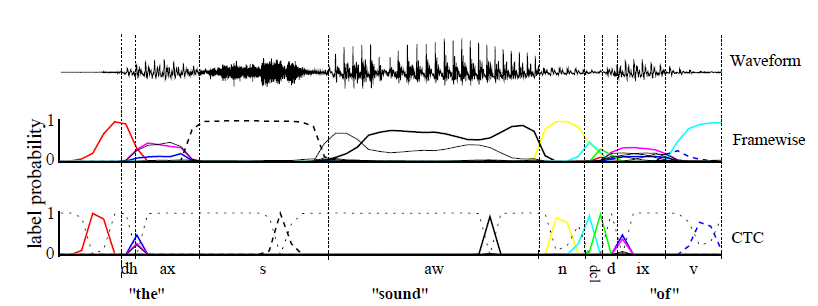
\includegraphics[width=1\linewidth]{pic/fig1} 

}

\caption{CTC and framewise classification networks applied to a speech signal}\label{fig:unnamed-chunk-1}
\end{figure}

有色线条是输出激活,对应于特定时间观察音素的概率。CTC网络只预测音素序列(通常为一系列尖峰,由``空白'',或空预测分隔,其概率以灰虚线表示。)然而framewise网络试图将它们与手动分割(垂直线)对齐。

\chapter{从输出到标签}\label{From-Outputs-to-Labellings}

\section{符号表示}

\begin{itemize}
\item
  \(y_k^t\) 表示输出序列在第 \(t\) 步的输出为 \(k\)
  的概率,举个简单的例子:(a-ab-),\(y_a^3\)
  表示在第3步输出的字母为a的概率
\item
  \(p(\pi|x)\) 表示给定输入 \(x\),输出为路径 \(\pi\)的概率。
\end{itemize}

假设在每个时间步输出的label的概率是相互独立的或条件独立的,那么\(p(\pi|x)\)
可以用公式是表示:\(p(\pi|x)=\prod_{t=1}^T(y_{\pi_t}^t)\),可以理解为每一个时间步输出路径为\(\pi_t\)的相应label的概率乘积。

\begin{itemize}
\item
  \(F\): 代表多对一的映射,将输出路径 \(\pi\) 映射到标签序列
  \(l\)的一种变换,这里忽略掉重复的label和空格,即
  \(F(a-aab-)=F(-aa-abb)=aab\)
\item
  \(p(l|x)\):表示给定输入\(x\),输出序列\(l\)的概率,因此输出序列\(l\)的概率可以表示为所有输出的路径
  \(\pi\)映射后的序列为 \(l\)
  的概率之和(因为路径之间是互斥的),公式表示为:
  \[p(l|x) = \sum_{\pi \in F_{(l)}^{-1}}p(\pi|x)\]
\end{itemize}

在同一个标签上折叠不同的路径,使得CTC使用未分段的数据成为可能,因为他允许网络预测标签而不事先知道他们发生的位置。这样在理论上使得CTC不适合必须事先确定标签的任务,而实际上从很多例子上发现CTC对于位置的预测也很准确。

\section{空格的作用}

最开始的CTC设定中是没有空格的,\(F\)只是简单的溢出了连续的相同字母,但是这样会产生两个问题:

\begin{itemize}
\item
  无法预测出连续两个相同的字母的单词了,比如说hello这个单词,在CTC中会删除掉连续相同的字母,因此CTC最后预测出的label应该是helo
\item
  无法预测出一句完整的话,而只能预测单个的单词。因为缺乏空格,CTC无法表示出单词与单词之间停顿的部分,因此只能预测出单个单词,或者将一句话中的单词全部连接起来了(这是对于英文而言)
\end{itemize}

因此,空格在CTC中的作用还是十分重要的。

\section{双向或单向网络}

假设CTC中使用的标签概率被假设为条件在整个输入序列上,喜欢双向(eg.BLSTM)RNN体系结构似乎是自然的。如果网络是单向的,在t时刻的label的概率只依赖于t时刻的输入。因此,在生成相应的标签之前,网络必须等到给定的输入段完成后(或至少充分地被识别)才可以。回想一下,对于framewise分类,对于每个输入具有单独的目标,将未来上下文合并到单向网络中的一种方式是在输入和目标之间引入延迟。单向CTC网络要更好一些,因为延迟不是固定的,而是可以由网络根据被标记的段来选择。在真实的应用场景中,使用单向的而非双向的网络造成的性能损失,CTC确实要比framewise要小。这对于应用(如实时语音识别)来说是值得考虑的,因为在这种场景下双向RNN可能是不适用的或不可能应用的。图2.1反映了单向和双向CTC网络的一些不同。

\begin{figure}

{\centering 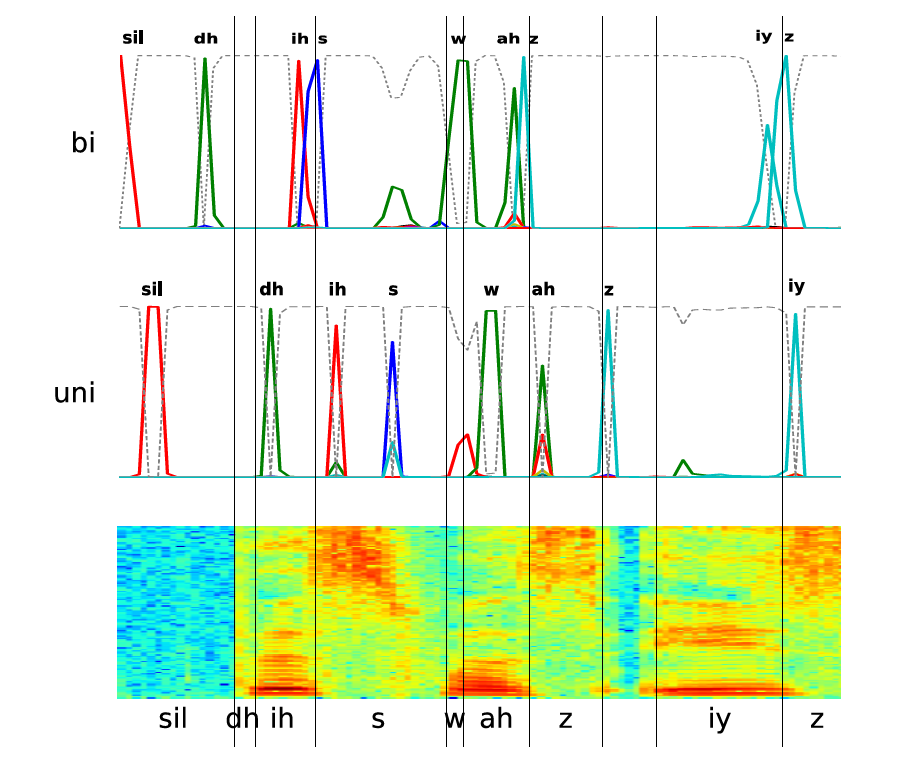
\includegraphics[width=1\linewidth]{pic/fig2} 

}

\caption{Unidirectional and Bidirectional CTC Networks}\label{fig:unnamed-chunk-2}
\end{figure}

\begin{itemize}
\item
  谱图(底部)代表话语的开始,其中由垂直黑线标记的手分段音素边界,以及下方的正确的语音标签。
\item
  输出音素概率由实线表示,而虚线则对应于``空白''概率。
\item
  单向网络(中间)和双向网络(上方)都成功地标记数据。
\item
  然而,它们在不同时期发出标签。
\item
  而单向网络必须等到相应的段完成后(例外是`sil'和`s',大概是因为它们需要较少的上下文来识别),双向网络可以在分段之前、之后或期间发射标签。
\item
  另一个重要的特点是双向CTC网络,善于把一些频繁协同发生的词粘合在一起(比如这里的`ah'和``z'',他们结合在``was''的押韵声中)
\end{itemize}

\chapter{前向传播与反向传播}\label{Forward-Backward-Algorithm}

我们来看一下CTC是怎样训练的\ldots{}\ldots{}

在对符号做了一些定义之后,我们接下来看看CTC的前向传播的过程。我们前向传播就是要去计算
\(p(l|x)\) 由于一个序列 \(l\)
通常可以有多条路径经过映射后得到,而随着序列 \(l\)
长度的增加,相对应的路径的数目是成指数增加的,因此我们需要一种高效的算法来计算它。

有一种类似于HMM的前向传播的算法可以帮助我们来解决这个问题。它的关键点就是那些与序列
\(l\) 对应的路径概率都可以通过迭代来计算得出。

\section{前向传播}

对于一个特定的序列\(l\)
,我们定义前向变量\(\alpha(t,u)\)为输出所有长度为\(t\),且经过\(F\)
映射之后为序列\(l\) 的路径的概率之和,用公式表达如下所示:
\[\alpha(t,u)=\sum_{\pi \in V(t,u)}\prod_{i=1}^{t}y_{\pi_i}^{i}\]
其中\(V(t,u)=\{\pi \in A^{'T}:F(\pi)=l_{1:u/2},\pi_t=l_u^{'}\}\)
代表了所有满足经过 \(F\) 映射之后为序列\(l\)
,长度为t的路径集合,且在第t时间步的输出为label:
\(l_u^{'}\).注意这里的\(l^{'}\)是对\(l\)进行空白插入得到的,且插入后的维度定义为\(U^{'}=2U+1\),其中\(U\)表示\(l\)的长度。

正如我们将看到的,在时间t的前向变量可以从时间t-1的递归计算。

所有正确路径的开头必须是空格或者label:\(l_1\),因此存在着初始化的约束条件:

\[\alpha(1,1) = y_b^1\]

\[\alpha(1,2) = y_{l_1}^1\]

\[\alpha(1,u) = 0 \quad \forall u>2\]

我们通过下图去理解这个过程:

\begin{figure}

{\centering 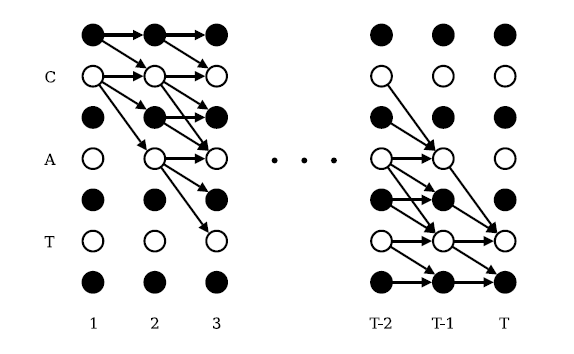
\includegraphics[width=1.5\linewidth]{pic/fig_3} 

}

\caption{CTC forward-backward algorithm}\label{fig:unnamed-chunk-3}
\end{figure}

上图中,白色的点表示一个label,黑色的点表示空格,纵向每一列表示的是路径的长度T(或者时刻T),箭头代表了路径下一个时刻可以输出到哪个label去。如果在时刻
1 的 label
为空格,那么路径在下一时刻只有两个选择,第一个还是输出空格,第二个就是输出序列
\(l_1\) 中对应的空格的下一个label:C;如果在时刻2的 label 为
C,那么在时刻3,它可以有三种选择:第一种就是输出还是
C,第二种是输出为空格,第三种是直接输出A。

从上图可以看出长度为T的输出路径映射到序列 \(l\):cat,
可以由第T步为label:t(cat中的字母t)的所有路径和第T步为空格的所有路径的概率之和来表示。

因此,\(p(l|x)\)可以由前向变量来表示,即为

\[p(l|x)=\alpha(T,U^{'})+\alpha(T,U^{'}-1)\]

其中\(\alpha(T,U^{'})\)可以理解为所有路径长度为\(T\),经过\(F\)映射之后为序列\(l\),并且第\(T\)时刻的输出的label为\(l^{'}_U\)或者\(l^{'}_{U-1}\)。也就是路径的最后一个是否包含了空格。

现在我们来引出其推导公式:

\[\alpha(t,u)=y_{l^{'}_u}^t\sum_{i=f(u)}^u\alpha(t-1,i)\]

其中

\begin{center}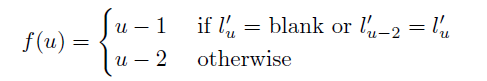
\includegraphics[width=1.5\linewidth]{pic/fig_5} \end{center}

\begin{verbatim}
$$
\begin{equation}
f(u)=\left\{
\begin{aligned}
& u-1  & if \quad l_u^{'}=blank \quad or \quad l_{u-2}^{'}=l_u^{'}\\
& u-2 & otherwise \\
\end{aligned}
\right.
\end{equation}
$$
\end{verbatim}

如何理解这个递推公式呢,很简单,我们可以看下面递推图,就以时刻T为空格的前向变量为例,由于我们之前讲过了如果当前时刻的输出为空格,下一时刻路径输出只有两种可能性,而如果我们当前时刻是空格,上一时刻的输出从图中可以看出也是由两种可能性,一种是在T-1时刻输出为空格,另外一种是在T-1时刻输出为T。因此我们只要计算出T-1时刻输出为空格的所有正确路径的概率之和以及在T-1时刻输出为T的所有路径的概率之和,再乘上T时刻输出为空格的概率
\(y_{l_u^{'}}^t\),就可以得到前向变量\(\alpha(t,u)\)。时刻T为label:T的前向变量的求法和空格的类似,只是它由三种可能情况求和再乘上
\(y_{l_u^{'}}^t\) 得到的。

详看下面的示意图:

\begin{figure}

{\centering 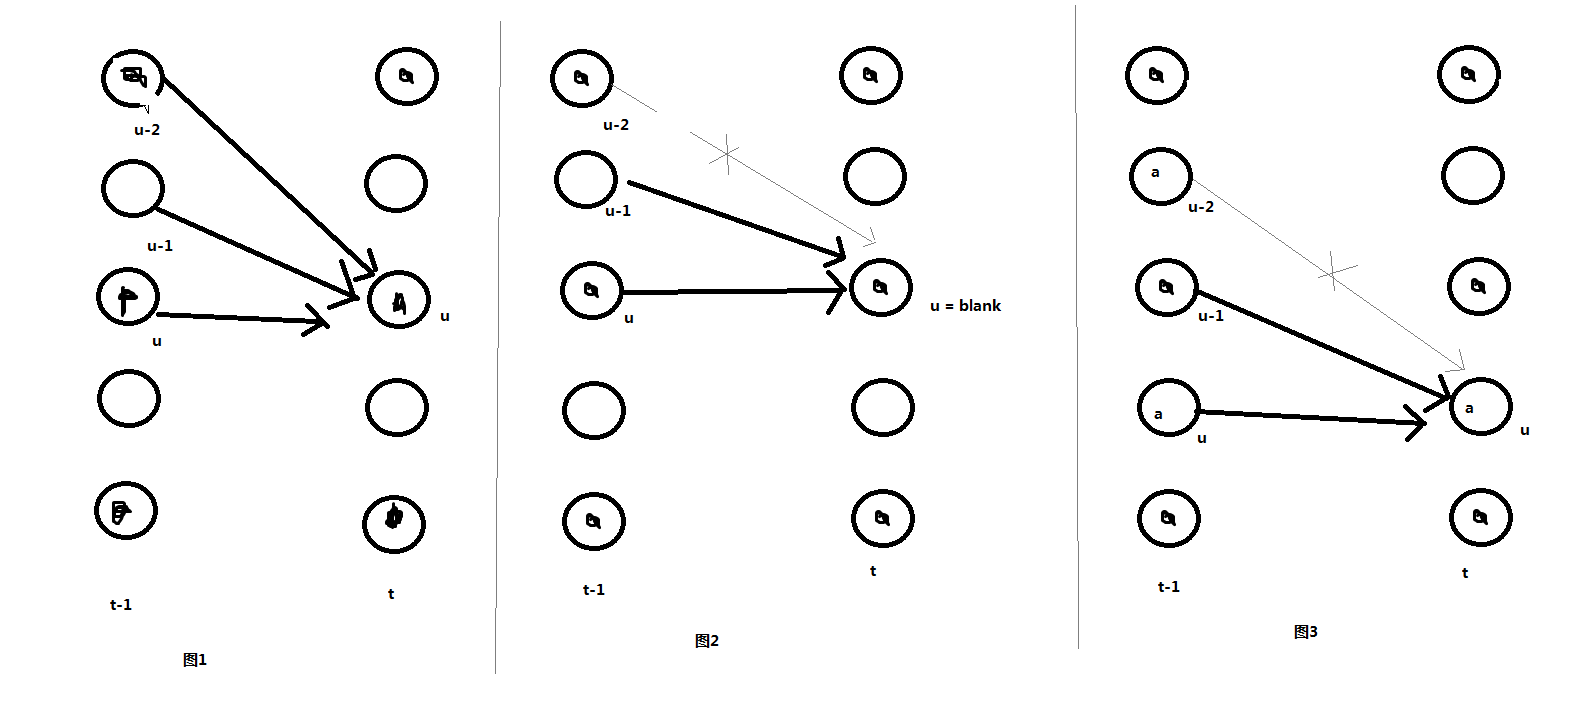
\includegraphics[width=1\linewidth]{pic/fig_4} 

}

\caption{CTC 递推关系示意图}\label{fig:unnamed-chunk-5}
\end{figure}

\section{反向传播}

与前向传播类似,首先定义一个反向变量\(\beta(t,u)\),他的含义是从\(t+1\)时刻开始,在前向变量\(\alpha(t,u)\)上添加路径\(\pi^{'}\),使得最后通过\(F\)映射之后为序列\(l\)的概率之和,用公式表示为:

\[\beta(t,u) = \sum_{\pi \in W(t,u)} \prod_{i=1}^{T-t}y_{\pi_i}^{t+i}\]

其中\(W(t,u) = \{\pi \in A^{'T-t}: F(\pi^{'}+\pi)=l, \forall \pi^{'} \in V(t,u) \}\)

按照前向传播的图的举例说明:假设我们在T-2时刻路径输出为label:A,那么此时的反向变量的求法是在T-2时刻开始,所有能到达T时刻输出为空格或者label:T的``剩余''路径\(\pi^{'}\)的概率之和。

反向传播也有相对应的初始化有条件:

\[\beta(T,U^{'})=\beta(T,U^{'}-1)=1\]
\[\beta(T,u^{'}) = 0, \quad \forall u^{'} < U^{'}-1\]

他的递推公式如下所示:

\[\beta(t,u) = \sum_{i=u}^{g(u)}\beta(t+1,i)y_{l_{i}^{'}}^{t+1}\]

其中

\begin{center}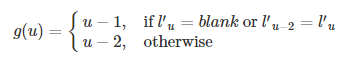
\includegraphics[width=1.5\linewidth]{pic/fig_6} \end{center}

\section{log尺度变换}\label{log}

在现实中,不论是计算前向变量还是计算反向变量,都会涉及到大量的概率乘积的运算,概率都是小于1的数进行乘积运算时计算机在处理时会使得趋于0的数近似于0(underflows:你可以在R中输入\texttt{(sqrt(2))\^{}2==2}就可以看到这种现象),因此做对数变换,变换完之后,变量中的加法运算就不方便了,然后就又用了一个trick:

\[\ln(a+b)=\ln a+ \ln (1+e^{\ln b - \ln a})\]

\chapter{损失函数}

\section{损失函数的定义}

\[L(S) = -\ln\prod_{(x,z)\in S} p(z|x) = -\sum_{(x,z)\in S} \ln p(z|x)\]

其中S为训练集。损失函数可以解释为:给定样本后输出正确label的概率的乘积,再取负对数就是损失函数了。取负号之后我们通过最小化损失函数(说白了就是一个似然函数损失),就可以使输出正确的label的概率达到最大了。

由于上述定义的损失函数是可微的,因此我们可以求出它对每一个权重的导数,然后就可以使用什么梯度下降系列的算法来进行优化求解。

下面我们就要把上一节定义的前向变量与反向变量用到我们的损失函数中去,令序列\(l=z\),
定义\(X(t,u)=\{\pi \in A^{'T}: F(\pi)=z\pi_t=Z_u^{'}\}\),\(X(t,u)\)代表了在时刻t进经过label:\(l_u^{'}\)的所有路径的集合,这样由之前对前向变量和后向变量的定义,他俩的乘积就可以写成:

\[\alpha(t,u)\beta(t,u) = \sum_{\pi \in X(t,u)} \prod_{t=1}^Ty_{\pi_t}^t\]

而\(p(\pi|x)=\prod_{t=1}^T(y_k^t)\),因而进一步转化可以得到:

\[\alpha(t,u)\beta(t,u) = \sum_{\pi \in X(t,u)}p(\pi|x)\]

因此,对于任意时刻t,我们给定输入x,输出序列z的概率可以表示为:

\[p(z|x)=\sum_{u=1}^{|z^{'}|}\alpha(t,u)\beta(t,u)\]

也就是在任意时刻分开,前向变量和反向变量的乘积为在该时刻经过label:\(l_u^{'}\)的所有概率之和。

损失函数就改写为:

\[L(x,z) = -\ln \sum_{u=1}^{|z^{'}|}\alpha(t,u)\beta(t,u) \]

\section{损失函数的梯度计算(BPTT)}\label{bptt}

损失函数关于网络输出\(y_{k}^t\)的偏导数:

\[\frac{\partial L(x,z)}{\partial y_k^{t}}=-\frac{\partial \ln p(z|x)}{\partial y_k^{t}}=-\frac{1}{p(z|x)}\frac{\partial p(z|x)}{\partial y_k^{t}}\]

而\(p(z|x)=\sum_{u=1}^{|z^{'}|}\alpha(t,u)\beta(t,u)= \sum_{\pi \in X(t,u)} \prod_{t=1}^Ty_{\pi_t}^t\),我们记label:k
出现在序列\(z^{'}\)的所有路径的集合为:\(B(z,k)=\{u:z_u^{'}=k\}\),因而可以得到:

\begin{center}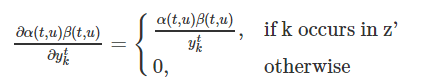
\includegraphics[width=1.5\linewidth]{pic/fig_7} \end{center}

即:

\[\frac{\partial p(z|x)}{\partial y_k^t}=\frac{1}{y_k^t}\sum_{u \in B(z,k)}\alpha(t,u)\beta(t,u)\]

可以得到损失函数对\(y_{k}^{t}\)的偏导数

\[ \frac{\partial L(x,z)}{y_{k}^{t}} = -\frac{1}{p(z|x)y_{k}^{t}}\sum_{u \in B(z,k)}\alpha(t,u)\beta(t,u)\]

最后:特别注意(softmax层)\[y_k^t = \frac{e^{a_k^t}}{\sum_{k^{'}}e^{a_{k^{'}}^t}}\]

我们就得到损失函数关于\(a_k^t\)的偏导数:

\[\frac{\partial L(x,z)}{\partial a_k^t}= -\sum_{k^{'}}\frac{\partial L(x,z)}{\partial y_{k^{'}}^t}\frac{\partial y_{k^{'}}^t}{\partial a_k^t}\]

\[\frac{\partial L(x,z)}{\partial a_k^t}= y_{k}^t-\frac{1}{p(z|x)}\sum_{u\in B(z,k)}\alpha(t,u)\beta(t,u)\]

注:最后式子的推导见附加页

可以使用BPTT算法得到损失函数对神经网络参数的偏导。

\chapter{Decoding}\label{decoding}

我们在第3章介绍了如何训练CTC,那么问题来了,给定输入序列\(X\)如何做预测?解码是对于输入序列\(X\)找出概率最大的输出序列\(l\),而不是概率最大的一条输出路径,因为输出路径和输出序列是多对一关系。

\[l^{*}=arg \quad max_{l}\quad p(l|x)\]

\section{Best Path Decoding}\label{best-path-decoding}

最优路径找出每一帧输出的最大概率组成的输出序列即为最后的解码结果。
他基于一个假设:最有可能的输出序列对应最有可能的标签。

\section{Prefix Search Decoding}\label{prefix-search-decoding}

是基于前向后向算法的改进。其标签序列对应HMM里面的状态序列。任意状态之间是可以相互转换的,由隐马尔可夫链决定转换成功率。而标签序列是有顺序的,所以只能从一个转换到下一个,而不能从下一个状态回到上一个状态。如图所示。只能先a后b,而不能先b后a。

\section{Constrained Decoding}\label{constrained-decoding}

对于语音识别,可以引入语言模型等grammar限制,求解问题变为如下形式。

\chapter{Example}\label{example}

\chapter{Discussion}\label{discussion}

\chapter{tensorflow API}\label{tensorflow-api}

\chapter{参考文献}

{[}1{]}.\url{https://blog.csdn.net/xmdxcsj/article/details/70300591}

{[}2{]}.\url{https://blog.csdn.net/left_think/article/details/76370453}

{[}3{]}.\url{https://blog.csdn.net/gzj_1101/article/details/80153686}

{[}4{]}.Supervised Sequence Labelling with Recurrent Neural
Networks(chapter7)

{[}5{]}.\url{https://distill.pub/2017/ctc/}

问题:

\begin{enumerate}
\def\labelenumi{\arabic{enumi}.}
\item
  简述CTC和传统的混合模型的主要区别?
\item
  思考CTC和HMM的区别和联系?
\end{enumerate}

\bibliography{book.bib,packages.bib}


\end{document}
